\documentclass[12pt]{article}

\usepackage[T1]{fontenc}
\usepackage[utf8]{inputenc}
\usepackage[russian]{babel}

% page margin
\usepackage[top=2cm, bottom=2cm, left=2cm, right=2cm]{geometry}

% AMS packages
\usepackage{amsmath}
\usepackage{amssymb}
\usepackage{amsfonts}
\usepackage{amsthm}

\usepackage{float}
\usepackage{graphicx}
\usepackage{tabularx}

\newcommand{\lb}{\left(}
\newcommand{\rb}{\right)}

\makeatletter
\setlength{\@fptop}{0pt}
\makeatother

\begin{document} 

\begin{titlepage}
\centering
\textbf{\large Московский государственный университет имени М.В.\,Ломоносова\\
\vspace*{0.1cm} Химический факультет\\
\vspace*{0.1cm}
\noindent\makebox[\linewidth]{\rule{\paperwidth}{0.4pt}}
\vspace*{0.1cm}
 Кафедра физической химии}
\vspace*{2cm}

\begin{center}

\includegraphics[width=0.3\textwidth]{pictures/logo.jpg}
\end{center}

\vspace*{2cm}
\Large \textbf{Сканирующая электронная микроскопия электропроводящих материалов}
\vspace*{6cm}

\begin{flushright}
\large Работа выполнена студентом 515 группы\\
Финенко А.А.\\
\end{flushright}
\vfill
\large\textbf{Москва\\ 2017}
\end{titlepage}


Термоэлектронная и автоэлектронная эмиссия. Катоды, применяемые в электронной спектроскопии. Основные характеристики, достоинства и недостатки. \par
\vspace{1cm}

Электронная пушка в сканирующем электронном микроскопе является источником пучка электронов, используемого для исследования поверхности образца. Электроны, испускаемые катодом, ускоряются электромагнитным полем и фокусируются на участке поверхности. Размер и форма катода, величина ускоряющего напряжения и интенсивность потока электронов являются преобладающими факторами, влияющими на разрешение, получаемое в сканирующей электронной микроскопии. \par
В основе работы электронной пушки лежит явление испускания электронов металлами в вакууме при высокой температуре или в сильном электрическом поле. В первом случае оно носит название \textit{термоэлектронной эмиссии}, а во втором -- \textit{автоэлектронной} или \textit{полевой эмиссии}. \par

\subsection*{Термоэлектронная эмиссия}
Если мы нагреем материал до достаточно высоких температур, то кинетическая энергия электронов может возрости до значений, превышающих величину энергетического барьера, удерживающего их внутри объема материала. Величина барьера для большинства материалов составляет несколько эВ. \par
Плотность термоэмиссионого потока, $j$, при температуре $T$ определяется законом Ричардсона
\begin{gather}
j = A T^2 \exp \lb - \frac{\Phi}{kT} \rb, \label{richardson}
\end{gather}

где $A \left[ A/ m^2 K^2 \right]$ -- постоянная Ричардсона, является характеристикой материала. Из вида уравнения видно, что существенный поток достигается, когда энергия теплового движения электронов $kT$ становится сопоставимой с энергетическим барьером $\Phi$. Поэтому подходящими материалами для термоэмиссионых источников являются либо материалы, обладающие высокой температурой плавления ($W$), или материалы, обладающие малым значением энергетического барьера $\Phi$ ($LaB_6$).

\subsection*{Автоэлектронная эмиссия}
Эффект автоэлектронной эмиссии заключается в испускании электронов с поверхности материала под действием электрического поля, которое искривляет потенциальный барьер, удерживающий электроны. При достаточном искривлении потенциального барьера электроны начинают туннелировать через барьер. Для искривления барьера необходимо создать огромную напряженность электрического поля, которая увеличивается как $\sim \displaystyle \frac{V}{r}$, где $r$ - радиус цилиндрического сечения материала. Так, из вольфрамовой нити делают иглу, радиус кончика которой не превышает $0.1 \mu m$. При приложении потенциала в 1 $kV$ напряженность поля в кончике составляет $\sim 10^{10} V/m$. \par
Для того, чтобы осуществлялась автоэлектронная эмиссия с поверхности материалы она не должна содержать загрязнителей или оксида. Этого достигают, помещая катод в высокий вакуум ($ < 10^{-9} Pa$); в этом случае катод функционирует в околокомнатных температурах. Кроме того, поверхность может быть сохранена в более низком вакууме, но в условиях нагрева поверхности. Такого типа катоды называются катодами Шоттки.

\subsection*{Вольфрамовый катод}

\begin{figure}[!ht]
\centering
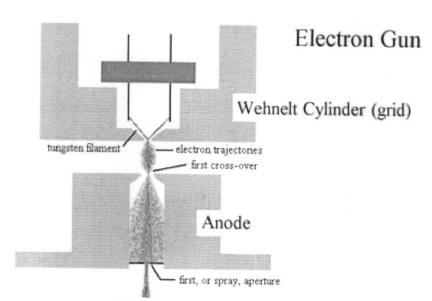
\includegraphics[scale = 0.5]{pictures/tungsten.png}
\caption{Электронная пушка с вольфрамовым катодом}
\label{tungsten-cathode}
\end{figure}

Источником электронного пучка в электронной пушке, изображенной на рис. \ref{tungsten-cathode}, является изогнутая вольфрамовая нить, диаметр которой приблизительно равен 100 мкм. Нить фиксируется металлическими штангами, пропущенными через керамическую подложку. Электрический ток, проходящий через вольфрамовую нить, нагревает ее и усиливает эффект термоэлектронной эмиссии. Оптимальная температура для выбивания термоэмиссионных электронов с поверхности вольфрамовой нити приходится на 2700 К. При помощи цилиндр Венельта (Wehnelt cylinder) к вылетащим электронам прикладывается ускоряющее напряжение, заставляющее последних покинуть область пространства вокруг нити. В отсутствии цилиндра термоэмиссионные электроны образовали бы заряженное облако вокруг нити, своим суммарным зарядом тормозящее дальнейшую эмиссию с нити.

\subsection*{Катод на основе гексаборида лантана}

\begin{figure}[!ht]
\centering
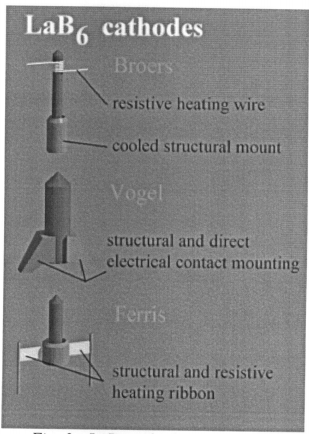
\includegraphics[width = 0.45\linewidth]{pictures/lantan.png}
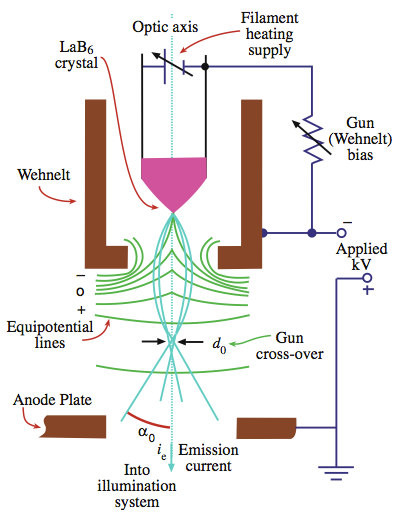
\includegraphics[width = 0.45\linewidth]{pictures/lantan1.png}
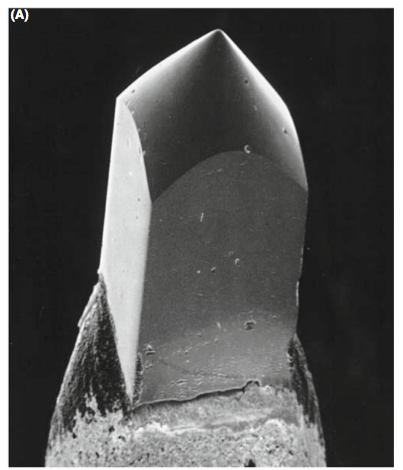
\includegraphics[width = 0.45\linewidth]{pictures/lantan2.png}
\caption{(сверху слева) Самые распространенные конструкции катодов со стержнем из $LaB_6$; (сверху справа) Схема конструкции электронной пушки с катодом из $LaB_6$; (снизу) кристалл $LaB_6$}
\label{lantan-rod}
\end{figure}

Другим источником катодов, используемых в электронной микроскопии, является стержень из гексаборида лантана $LaB_6$. Он представляет собой цельный кристалл порядка 1 мм в диаметре. Чтобы обеспечить нагрев этого катода до 1700-2100К было придумано несколько схем, представленных на рис. \ref{lantan-rod}. Конец стержня представляет собой небольшую скошенную площадку, с которой происходит равномерная эмиссия электронов. Катоды на основе $LaB_6$ обеспечивают яркость на порядке больше, чем вольфрамовые катоды. Однако для обеспечения их работы требуется более высокий вакуум.

\clearpage
\subsection*{Автоэмиссионные источники}

Автоэмиссионный катод представляет собой диод, в котором катодом является нить, обычно вольфрамовая, конец которой сильно вытянут и заострен. Существенным требованием для работы АЭК является высокий или ультравысокий вакуум. Время от времени требуется очистка катода путем реверсирования потенциала катода, либо нагревом до $\sim 5000 K$.

\begin{figure}[!ht]
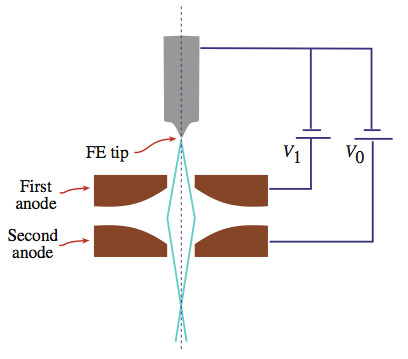
\includegraphics[width=0.5\linewidth]{pictures/feg1.png}
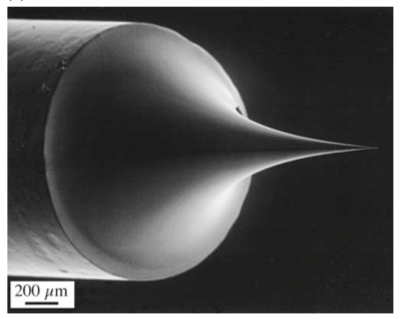
\includegraphics[width=0.5\linewidth]{pictures/feg2.png}
\caption{(слева) Схема электронной пушки с автоэлектронным катодом (справа) Кончик вольфрамового  автоэлектронного катода}
\end{figure}

Данные таблицы 1 показывают, что достоинствами катодов с автоэлектронной и термполевой эмиссиями является высокая яркость и плотность тока. Изображения, получаемые с помощью этих детекторов обладают большей четкостью и контрастностью. Кроме того, они более долговечны, чем термоэмиссионные катоды. Однако для их работы требуется более высокий вакуум.

\begin{table}[!ht]
\centering
\label{table1}
\begin{tabular}{cccccc}
& Единицы & $W$ & $LaB_6$ & Шоттки & холодные АЭ катоды \\
\hline
Работа выхода, $\Phi$ & eV & $4.5$ & $2.4$ & $3.0$ & $4.5$ \\
Константа Ричардсона, $A$ & $A / m^2 K^2$ & $6 \cdot 10^{9}$ & $4 \cdot 10^{9}$ & & \\
Рабочая температура, $T$ & $K$ & 2700 & 1700 & 1700 & 300 \\
Плотность тока, $j$ (100 kV) & $A / m^2$ & $5$ & $10^{2}$ & $10^{5}$ & $10^{6}$ \\
Яркость, (100 kV) & $A/m^2 sr$ & $10^{10}$ & $5 \cdot 10^{11}$ & $5 \cdot 10^{12}$ & $10^{13}$ \\
Вакуум & $Pa$ & $10^{-2}$ & $10^{-4}$ & $10^{-6}$ & $10^{-9}$ \\
Долговечность & $hr$ & $100$ & $1000$ & $>5000$ & $>5000$ \\
\hline
\end{tabular}
\caption{Параметры электронных источников}
\end{table}

\clearpage
\section*{Результаты эксперимента}

\begin{figure}[!ht]
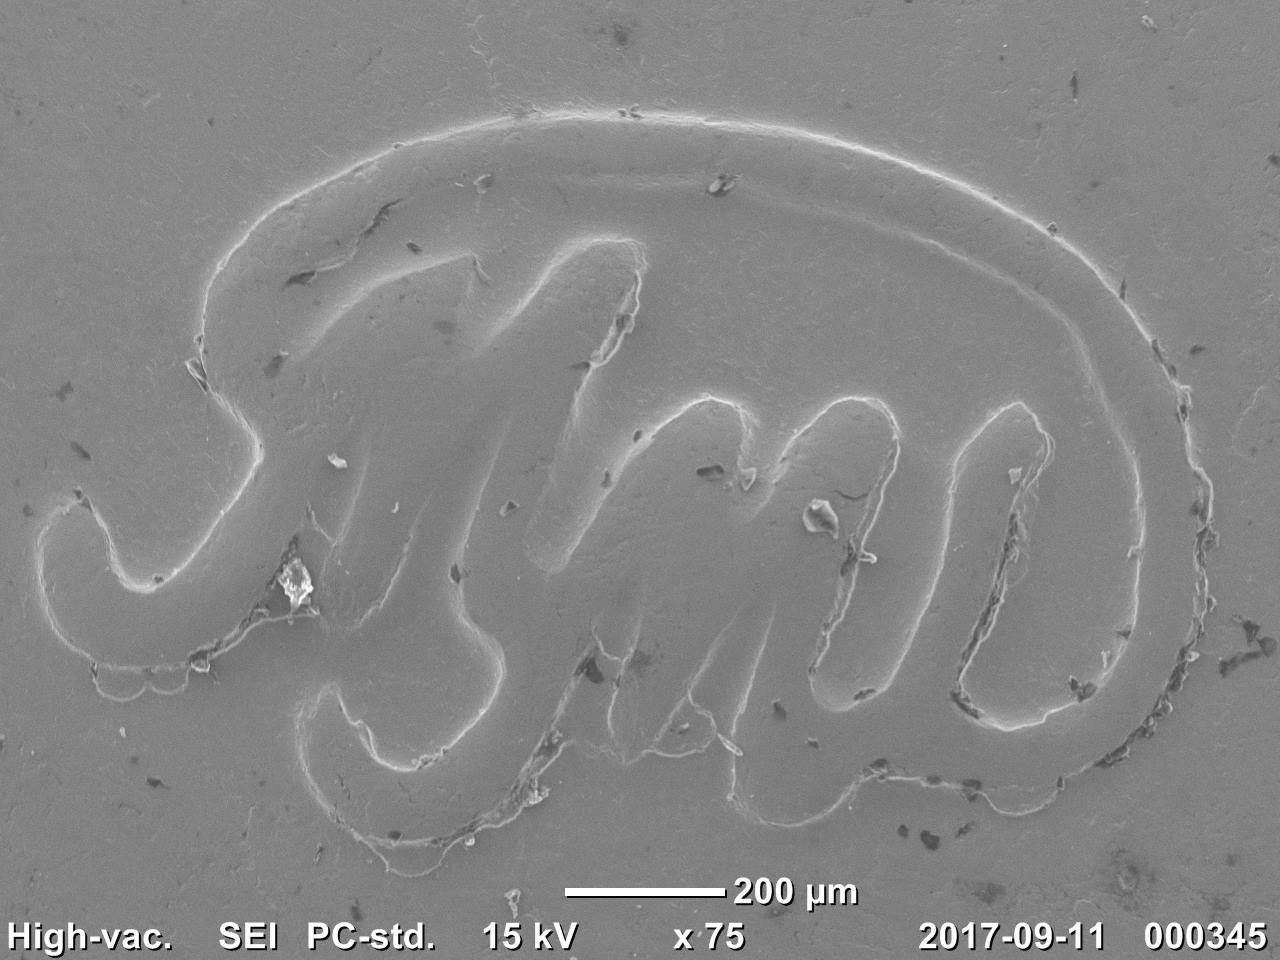
\includegraphics[width=0.5\linewidth]{pictures/20170911_000345.jpg}
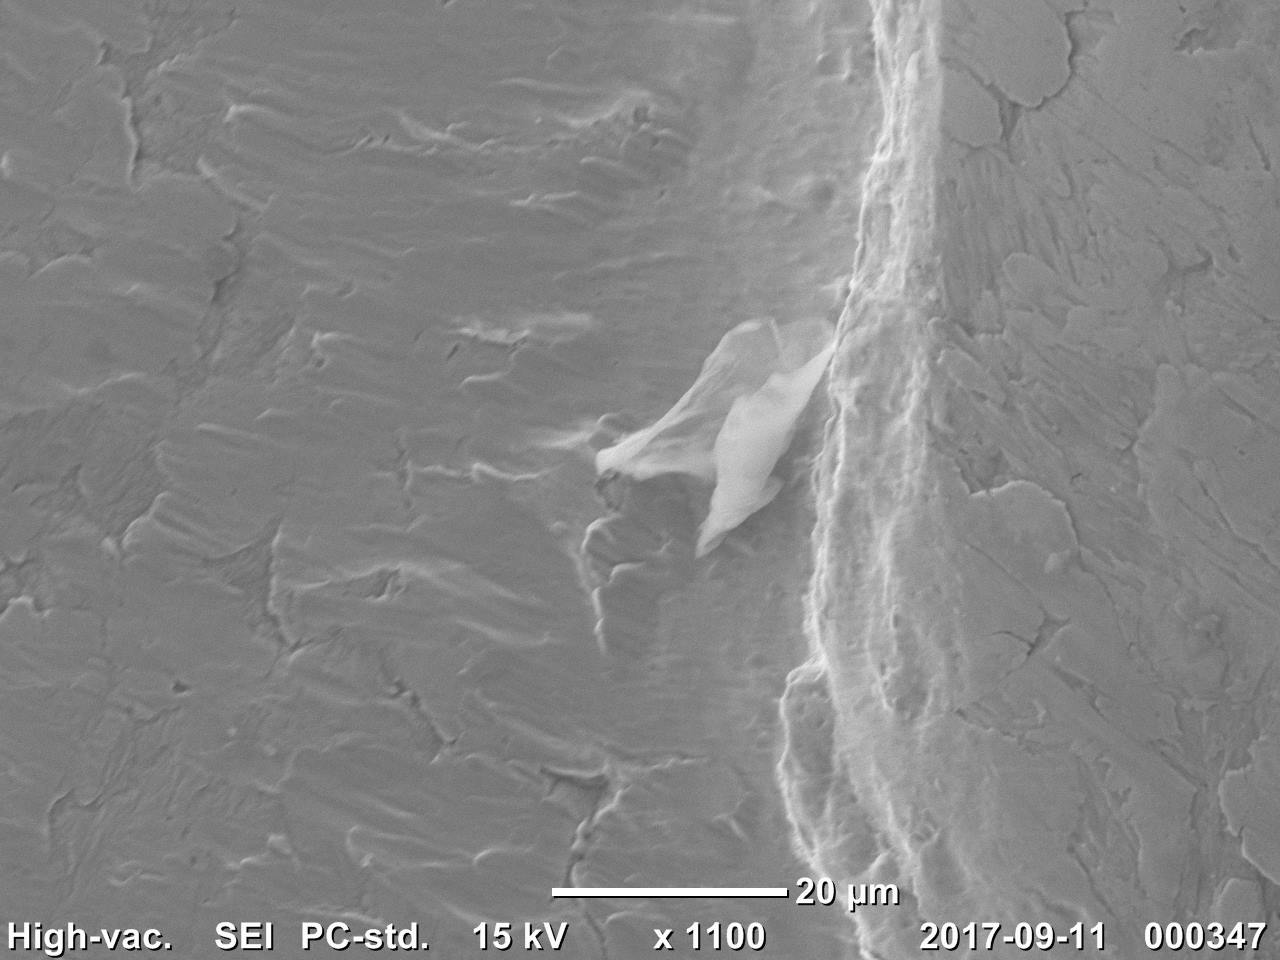
\includegraphics[width=0.5\linewidth]{pictures/20170911_000347.jpg}
\end{figure}

\begin{figure}[!ht]
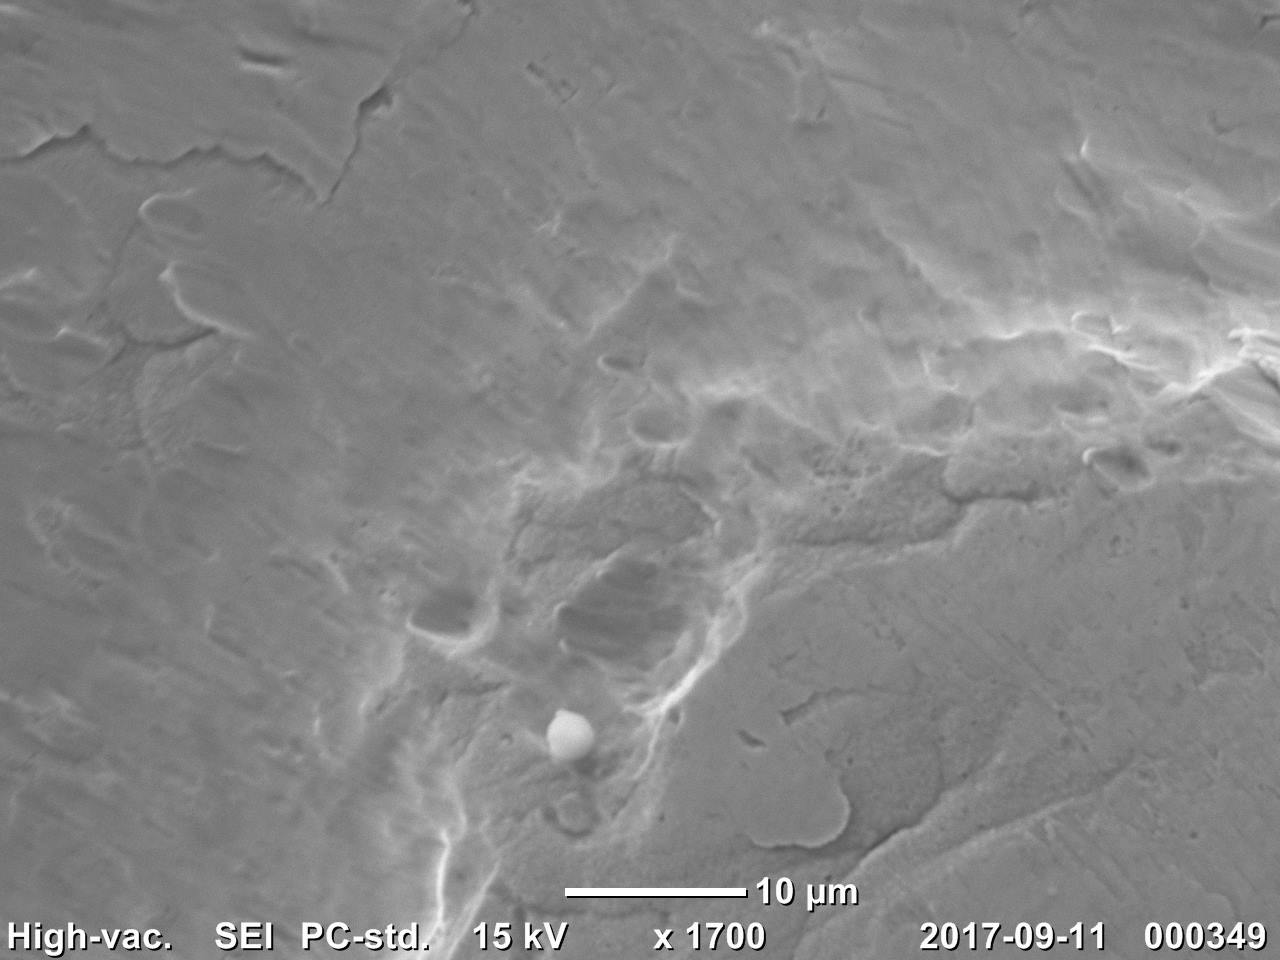
\includegraphics[width=0.5\linewidth]{pictures/20170911_000349.jpg}
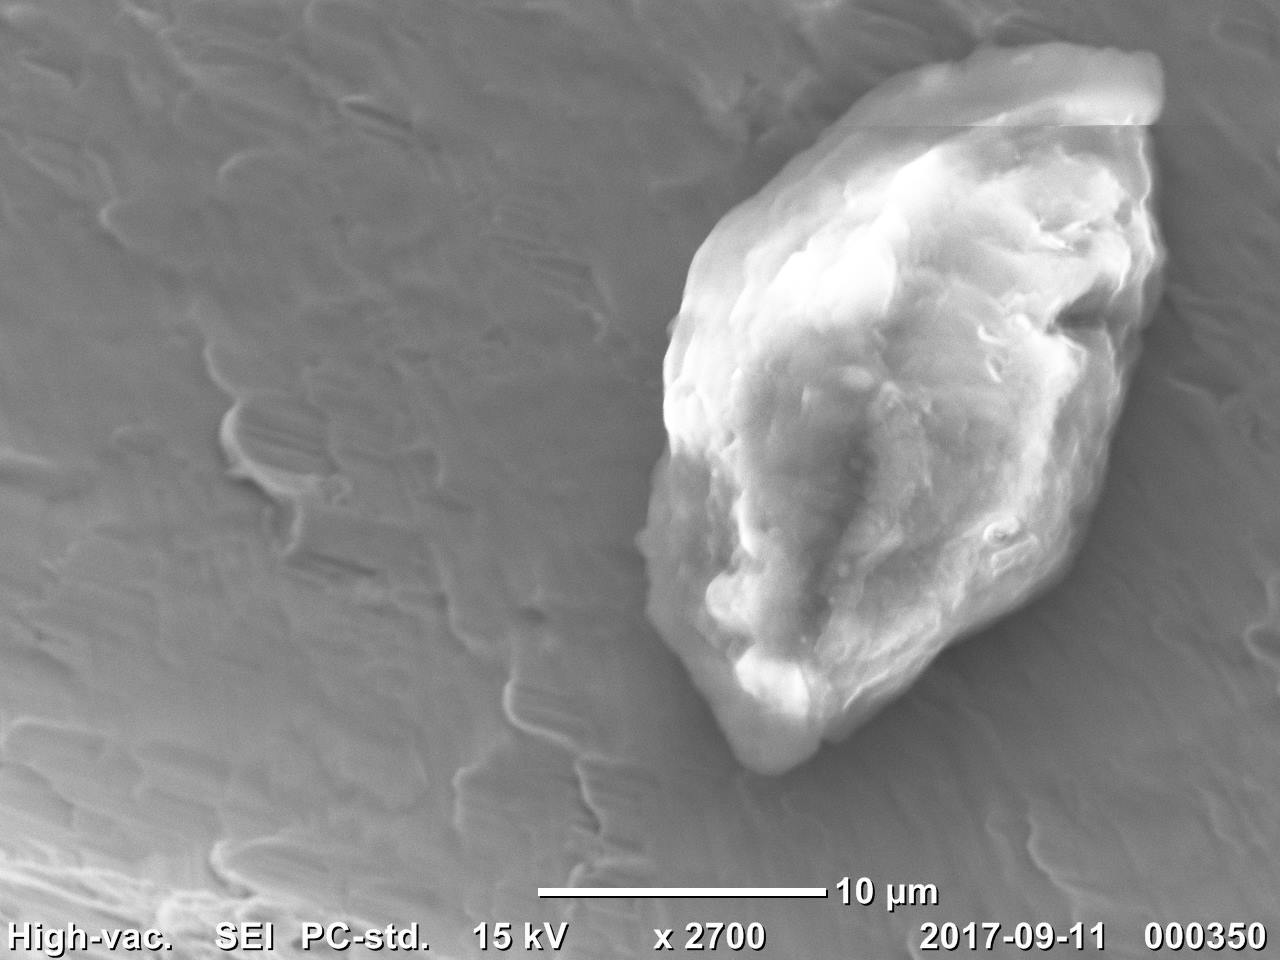
\includegraphics[width=0.5\linewidth]{pictures/20170911_000350.jpg}
\end{figure}

Объектом изучения является 10-рублевая монета банка России. Участки поверхности объекта были изучены при различных увеличениях. Все представленные снимки были сделаны с помощью детекторов вторичных электронов (SEI). На первом снимке представлен знак Московского монетного двора (ММД). На краях клейма видны существенные неоднородности металла. На последующих снимках представлены края изображения державы. \par
В режиме обратно отраженных электронов (BEI) контрастного изображения получить не удалось. Это вызвано тем, что контраст изображения при использовании детектора обратно отраженных электронов  возникает из-за неоднорости распределения электронной плотности на поверхности образца. В случае однородного элементного состава поверхности образца изображение получается малоконтрастным. Контраст при использовании детектора вторично рассеянных электронов (SEI) обусловлен рельефом поверхности образца. \par
Существенной зависимости качества изображения при малых значениях масштабного фактора от величины ускоряющего напряжения замечено не было (ускоряющее напряжение на используемом микроскопе может принимать значения 5, 10, 15 keV). При высоких значениях масштабного фактора контрастное изображение получалось только при наиболее высоком значении ускоряющего напряжения. Интенсивность электронного пучка может принимать три дискретных значениях, обозначенных в программном интерфейсе как PC-low, PC-std и PC-high. При наиболее высоком значении интенсивности электронного пучка наблюдается существенная засветка изображения. При среднем значении интенсивности при высоком значении масштабного фактора (и при медленном режиме съемки) наблюдается засветка изображения (изображение 000350). 


\section{Список литературы}

\begin{enumerate}
	\item Williams D. B., Carter C. B. (2009). Transmission Electron Microscopy: a Textbook for Materials Science. New York: Springer. 2nd ed.
	\item Goldstein, G. I., Newbury, D. E., Echlin, P., Joy, D. C., Fiori, C., Lifshin, E. (1981). Scanning electron microscopy and x-ray microanalysis. New York: Plenum Press. 
	\item Egerton, R. F. (2008). Physical Principles of Electronic Microscopy: an Introduction to TEM, SEM and AEM.	New York: Springer.  
\end{enumerate}

\end{document}


